\documentclass[oribibl]{llncs}
%\documentclass{llncs}
%\documentclass[citeauthoryear]{llncs}
%\documentclass[]{pasj01}
%\documentclass[draft]{pasj01}
%\documentclass[proof]{pasj01}
%\draft
%%%%%%%%%%%%%%%%%%%%%%%%%%%%%%%%%%%%%%%%%%%%%%%%%%%%%%%%%%%%%%%%
\usepackage{graphicx}
%\usepackage{listings}
\usepackage{comment}
\usepackage{color}
\usepackage{booktabs} % For formal tables
\usepackage{bm} % For formal tables
\usepackage{amsmath, amssymb}
\newcommand{\myvec}[1]{\vec{#1}}
\newcommand{\redtext}[1]{\textcolor{red}{#1}}

\newcommand{\icarus}{Icarus}
\newcommand{\pasa}{Publications of the Astronomical Society of Australia}
\newcommand{\aap}{Astronomy \& Astrophysics}
\newcommand{\aj}{The Astronomical Journal}
\newcommand{\apj}{The Astrophysical Journal}
\newcommand{\apjl}{The Astrophysical Journal Letters}
\newcommand{\mnras}{Monthly Notices of the Royal Astronomical Society}
\newcommand{\nat}{Nature}
\newcommand{\pasj}{Publications of the Astronomical Society of Japan}

%%%%%%%%%%%%%%%%%%%%%%%%%%%%%%%%%%%%%%%%%%%%%%%%%%%%%%%%%%%%%%%%

\begin{document}

\title{Parallel Algorithms for Global Simulation of Planetary Rings on
  Ultra Many Core System}

\author{Masaki Iwasawa \inst{1} \and Long Wang \inst{1, 2} \and Keigo
  Nitadori \inst{1} \and Daisuke Namekata \inst{1} \and Takayuki
  Muranushi \inst{1} \and Miyuki Tsubouchi \inst{1} \and Junichiro
  Makino \inst{1, 3, 4} \and Zhao Liu \inst{5} \and Haohuan Fu
  \inst{6} \and Guangwen Yang \inst{7}}

\institute{RIKEN Advanced Institute for Computational Science,
  7--1--26 Minatojima--minami--machi, Chuo--ku, Kobe, Hyogo, Japan
  \and Helmholtz Institut f\"{u}r Strahlen und Kernphysik, Nussallee
  14--16, D--53115, Bonn, Germany \and Department of Planetology,
  Graduate School of Science, Kobe University, 1--1, Rokkodai--cho,
  Nada--ku, Kobe, Hyogo, Japan \and Earth--Life Science Institute,
  Tokyo Institute of Technology, 2--12--1 Ookayama, Meguro--ku, Tokyo,
  Japan \and National Supercomputing Center in Wuxi, Wuxi, China \and
  Department of Earth System Science, Tsinghua University, Beijing,
  China \and Department of Computer Science and Technology, Tsinghua
  University, Beijing, China}

\maketitle

\begin{abstract}

In this paper, we report the efficient paralle $N$-body algorithms for
global simulation of planetary rings system and the measured
performance of the ring sinulation wiht up to 8 billion particles on
up to 2048 nodes (8192 processes) of TaihuLight. The measured
performance is around 35\% of the theoretical peak, while the
efficiency of the interaction kernel is currently around 50\%.
general considerations on performance optimization on heterogeneous
systems such as TaihuLight.

\end{abstract}

\section{Introduction}
\label{sect:intro}

Saturn's ring was found by Galileo Galilei in 1610. For more than
three centuries, it had been the only known ring system within our
solar system. In 1977, Rings of Uranus were found through ground-based
observations, and then in 1979 Rings of Jupiter by Voyager 1 and in
1989 those of Neptune by Voyager 2.  Very recently, it turned out that
some of minor planets also have rings. The first distinctive example
is 10199 Chariklo, whose orbit is between those of Saturn and Uranus
(and thus one of Centaurs). There are probably more Centaurs with
rings.

Recently, it was announced that a very large and complex ring system
is found around an planet of a star ``1SWASP J140747.93-394542.6''
\cite{2012AJ....143...72M, 2014MNRAS.441.2845V, 2015MNRAS.446..411K,
  2015ApJ...800..126K}. In April and May 2007, the star showed quite
complex change of brightness, which was interpreted as the result of
eclipses of the star by the planetary rings. If this interpretation is
correct, the ring is huge, with the outer radius of 90 million km (0.6
AU). For comparison, Saturn's F Ring has the radius of $1.4\times
10^5{\rm km}$, and even the outer radius of the very faint E ring is
less than $5\times 10^5{\rm km}$.  Thus, quite recently, a wide
variety of ring systems have been found.  How these rings are formed
and have evolved is an important question in planetary science.

Our understanding of the structure of the rings have been advanced
greatly, mainly through interplanetary missions such as Voyager 1 and
2, and most recently Cassini. Through these missions, a number of new
findings have been made. Among the new findings, probably the most
surprising is that the rings show dynamic changes of structures,
possibly including the formation of new satellites. Another example of
truly new findings of the Cassini mission is the vertical structure at
the outer edge of the B ring.  Other new findings include axisymmetric
structures of a vast range of scales, from 100m to 100km.

For some of these new findings, theoretical explanation based on fluid
approximation has been made. However, many of them cannot be explained
with simple fluid models, and more realistic treatment of ring as
collection of particles interacting through both mutual gravity and
physical collisions is necessary.

Planetary rings are usually at the radii around the Roche limit. Thus,
mutual gravity between particles does not easily lead to the formation
of new satellites, but is important enough to form spiral waves
(``wakes'') in very small scales, which increases the effective
viscosity and should enhance the radial transport of the angular
momentum. On the other hand, the actual ring system seems to consist
of very large number of very narrow rings, separated with distinct
gaps. It is believed that high-order resonances with small embedded
satellites (so-called moonlets), but whether or not such gaps can be
formed by resonances has not been fully understood.

Very little simulation-based studies have been done to understand
these new findings. The primary reason for this lack is simply that
simulations of such structures must be global simulations including
self gravity of ring particles, which would require very large number
of particles and thus very large amount of computing resources.

Up to now, most of simulations of ring structures have been local
ones, in which a small patch was cut out from the ring and simulated
under the assumption of the local Hill approximation and periodic
boundary condition \cite{1988AJ.....95..925W}.

Rein and Latter (2013) performed ``Large-scale'' simulation of viscous
overstability in Saturn's rings, using up to 204,178 particles and up
to 10,000 orbits using this local approach
\cite{2013MNRAS.431..145R}. Because very long simulations are
necessary, the number of particles has been small. They used {\tt
  REBOUND} \cite{2012A&A...537A.128R} , an MPI-parallel $N$-body
simulation code. More recently, Ballouz et al. (2017)
\cite{2017AJ....153..146B} used {\tt pkdgrav}
\cite{2001PhDT........21S} for simulations with up to 500k particles.

Compared to the size of local simulations performed so far, the number
of particles necessary for global simulations might seem too
large. However, such large simulations are not beyond the reach of
present-day supercomputers.

We have developed a framework for developing fast and highly scalable
codes for particle-based simulations, FDPS (Framework for Developing
Particle Simulator) \cite{2016PASJ...68...54I}. Using FDPS, Michikoshi
and Kokubo (2017) \cite{2017ApJ...837L..13M} performed global
simulations of rings with probably the largest number of
particles. They used 300M particles to model two narrow rings of
Chariklo and followed the system for 10 orbital period. The number of
particles they used is already three orders of magnitude larger than
what have been used for global simulations. They have used Cray XC30
at the Center of Computational Astrophysics, National Astronomical
Observatory of Japan, with the peak speed of 1 Pflops. In order to
model fine structures of Saturn's rings, we need to increase the
number of particles by another three orders of magnitude.

The total calculation cost is roughly proportional to number of
particles multiplied by the number of orbital periods followed, since
the calculation cost per timestep is $O(N \log N)$ when Barnes and Hut
tree algorithm is used and the number of timestep required for ring
simulations is essentially independent of the number of
particles. Thus, we can conclude that the size of state-of-the-art
simulations of planetary rings is around $3 \times 10^9$
particle-orbits, or around $3 \times 10^{12}$ particle-steps.

We should note that even though the simulations so far done in this
field is relatively small, that does not mean there is no need or
possibilities for larger scale simulations. If we want to model the
global structures of rings, we cannot rely on local treatment. For
example, the effect of resonances with small satellites can only be
studied using global simulations. On the other hand, the number of
particles one need for global simulations, even for a very narrow
radial range, is very large. For example, consider A ring of Saturn
with the radius of around $1.3\times 10^5\rm km$. The typical radius
of ring particles is 6 m \cite{1985Icar...64..531Z}, and the optical
depth of the ring is around unity. Thus, we need $10^4$ particles per
$\rm km^2$ or around $10^{12}$ particles for the radial range of 100
km. With this radial range, we can model many of fine features
observed by Cassini directly.

If we could use particles with larger size, we could reduce the number
of particles required significantly. However, that would change the
viscous diffusion timescale of the ring, and thus what would be
observed. Thus, if at all possible, it is desirable to perform
simulations with particle of real physical radius, which would require
at least $10^{16}$ and ideally $10^{19}$ particle steps.

In other fields of astrophysics, very large simulations have been
performed. For example, Ishiyama (2014) \cite{2014ApJ...788...27I}
used $4096^3$ particles to follow the formation and growth of dark
matter halos of smallest scales. This simulation corresponds to
$10^{16}$ particle steps. Part of this calculation was performed on K
computer. The performance of K computer is $4.0\times 10^{10}$
particle steps per second on the entire K computer, or 60,000 particle
step per second per core for a processor core with the theoretical
peak performance of 16 Gflops \cite{Ishiyama2012} . The efficiency
they achieved is 55\% of the theoretical peak.

B{\'e}dorf et al. (2014) \cite{2014hpcn.conf...54B} performed the
simulation of Milky Way Galaxy using $2.42 \times 10^{11}$ particles
on large-scale GPGPU clusters. The achieved performance is 24.77
Pflops on ORNL Titan, and one timestep took 5.5 seconds. Thus they
have achieved the performance of $4.4 \times 10^{10}$ particle steps
per seconds. The theoretical peak performance of Titan is 73.2 Pflops
in single precision. Thus, the achieved efficiency is 33.8\%.

The current super computers are powerful enough to perform a realistic
global ring simulation. Thus we are trying to revile the mechanisms of
formation of ring structures of the Saturn using the global ring
simulation.

As a first step of the investigation of the ring formation, we propose
efficient algorithms of global ring simulations and port them to
FDPS. To develop the algorithms we use Sunway TaihuLight which is the
first ranked on the top 500 list on Nov. 2017. Since its processor
(SW26010) is heterogeneous manycore archetecture, our algorithms work
well not only on single or multi core based system, but also on
manycore systems.

In this paper, we report that the modification of algorithms of FDPS
for the global planetary ring simulations the measurement of its
performance on Sunway TaihuLight. The paper is organized as
follows. In section~\ref{sec:TaihuLight}, we briefly describe manycore
systems, especially the features of the Sunway TaihuLight system and
its SW26010 processor. In section~\ref{sec:impl0}, we briefly review
the original implementation of FDPS and the problems with the
planetary ring simulation on TaihuLight. In section~\ref{sec:impl1},
we describe the algorithms we developing. In section~\ref{sec:result},
we present the measured performance on TaihuLight. In
section~\ref{sec:result}, we summarize the results.



\section{Manycore System}
\label{sec:TaihuLight}

Recently, super computers installing manycore processors, such as
SW26010, GPU, Xeon-Phi and PEZY-SC are widely used in the field of
HPC.  For example, in Nov. 2008 only one manycore was on the top 500
list, but in Nov. 2017, about 100 systems have manycore processors on
the list. Especially, eight systems in top 10 have many core systems
in Nov. 2017.

One reason of the increase of using manycore porcessors is low power
consumption of manycore processors compared to single or multi core
processors. Power consumption of super computers have become a issue
over ten years, in the point of view of running cost and enviromental
protection. Thus Manycore system would become more inportant in the
field of HPC.

Sunway TaihuLight system is one of the manycore systems. It consists
of 40960 nodes, connected by the network with injection bandwidth of
8GB/s per node. The hardware network bandwidth is large enough for our
purpose.

The processor itself consists of four CGs (core groups), each with one
MPE (management processing element) and 64 CPEs (computing processing
elements). Both MPE and CPE are 64-bit RISC cores. MPE has L1 cache
memories for both instructions and data, and also L2 data cache. On
the other hand, each CPE has L1 instruction cache and 64KB of local
data memory. CPEs can communicate with the main memory through DMA.
Each CPE can initiate multiple asynchronous DMA operations. Thus, it
is possible to write the kernel loop so that the computation, DMA read
for the data which will be necessary for the next iteration, and DMA
write operation of the result of the previous iteration all run
concurrently and thus the communication with the main memory is
completely hidden. This capability of explicit control of
communication with main memory is crucial for achieving high
efficiency, as will be discussed in section \ref{sect:innovation}.

Each core group is connected to 8GB DDR3 DRAM with the theoretical
peak transfer rate of 34GB/s. The processor runs at the clock
frequency of 1.45GHz, and each core (both MPE and CPE) can perform
four double precision FMA operations. Thus, the theoretical peak
performance of one processor is 3016 Gflops and that of one CG is 754
Gflops.

CPEs in one CG are organized into an $8\times 8$ array, and within
each row or column, low-latency, high-bandwidth point-to-point and
broadcast communications are supported.

Operating system runs on MPE, and by default the user program also
runs on MPE. In order to use CPEs, there are two ways. One is to use
an extension of OpenACC designed for SW26010 processor, and the other
is use a lightweight thread library called Athread. Athread is more
difficult to use compared to OpenACC, but allows fine-grained control
of CPEs.

\section{Original Implementation of FDPS}
\label{sec:impl0}

In this section, we describe the original implementation of FDPS.

The following gives the steps for parallel Barns-Hut tree code when
using FDPS on CPU-based super computer.

\begin{enumerate}

\item Perform domain decomposition.
  
\item Exchange particles so that particles belong to appropriate
  domains.
  
\item Construct the ``local'' tree structure from particles in the
  domain.

\item Calculate physical quantities of the tree cell of the local tree.

\item Collect the information necessary for the calculation of
  interaction from other processes (so called local essential tree).
  
\item Construct the ``global'' tree from the collected information.

\item Calculate physical quantities of the tree cell of the global tree.

\item For small group of particles, construct the interaction list
  during traverse the tree. \label{enum:make_list}
  
\item Calculate interactions on the particles from particles in the
  interaction list. \label{enum:calc_force}

\item Repeat steps \ref{enum:make_list} and \ref{enum:calc_force}
  until forces on all partcles are done.
  
\item Integrate the orbits of particles.

\item Go back to step 1.
  
\end{enumerate}

For GPGPUs, FDPS version 2.0 or later also adopt the extension of this
algorithm, in which multiple pairs of this group and list are
constructed and then passed to GPGPU \cite{Hamadaetal2009}. In this
algorithm, all computations, except for the actual interaction
calculation in the double loop, is done on general-purpose front-end
computer. In addition, during the interaction calculation on GPGPUs,
MPE constructs the next interaction lists. Thus we can hide
constructing interaction list.

If we use this algorithms on Sunway TaihuLight, CPEs are used only for
interaction calculations and the other parts are done on
MPEs. However, this algorithm is not sufficient on Sunway
TaihuLight. This is simply because MPE is too slow compared with
CPEs. The execution time for MPE to perform the tree construction and
tree traversal is more than 10 times longer than that for CPEs to do
the interaction calculation, if the efficiency of the interaction
kernel is reasonably high 30-50\%. The same problem would occur even
if we use CPU-GPU heterogeneous systems with the performance ratio of
CPU to GPU is small.

B{\'e}dorf et al. \cite{2014hpcn.conf...54B}, avoid this problem by
porting all procedures to GPU side. However, even when this approach
is adopted, getting reasonable efficiency turned out to be not easy,
since then the performance of tree construction and tree traversal
would be limited by the bandwidth of the main memory for random
access.  Thus, traditional approach for Barnes-Hut tree algorithm is
not sufficient for manycore processors.

Thus, it is necessary to introduce some new approach to reduce the
calculation (or main memory access) cost of operations other than the
interaction calculation. We adopted the neighbor-list method used in
molecular-dynamics simulations with short-range interactions, in which
the list constructed before is persistently used for multiple steps
(hereafter we call this method persistent-list method). In next
section, we will describe this method.

\section{FDPS for Planetary Ring Simulation on Many Core System}
\label{sec:impl1}

In this section, we describe algorithms we modified FDPS for
simulating self-gravitating planetary ring on TaihuLight.

\subsection{Persistent List Method}
\label{subsec:list}

In the global ring simulations, each particle moves on nearly Kepler
orbit and a logical structure of the tree is similar for a shear time
scale of Kepler ring. Thus we can persistently use the same tree
structure and the interaction list for multiple timesteps.

By using this persistent interaction list, we can reduce the
calculation cost of the part other than the interaction calculation
drastically. While we are using the same interaction list, we skip the
domain decomposition, exchange of particles, construction of the local
tree. We still need to update the physical quantities of the cells of
the local tree, since particles in the lowest level have moved. Then,
using the list of nodes for the local essential tree, the
communication between the nodes is performed. Finally, the physical
quantities of the global tree is updated, and the force calculation is
performed using this updated global tree and the persistent
interaction list.

The steps of persistent list method is as follows.

\begin{enumerate}

\item Perform domain decomposition. \label{enum:1st_step_beg}
  
\item Exchange particles so that particles belong to appropriate
  domains.
  
\item Construct the ``local'' tree structure from particles in the
  domain.

\item Calculate physical quantities of the tree cell of the local
  tree.
  
\item Collect the information necessary for the calculation of
  interaction from other processes [so called local essential tree
    (LET)] and memorize LETs and their destination
  processes. \label{enum:LET}
    
\item Construct the ``global'' tree from the collected information.

\item Calculate physical quantities of the tree cell of the global tree.
  
\item For small group of particles, construct the interaction list and
  memorize it during traverse the tree.
  
\item Calculate interactions on the particles from particles in the
  interaction list.

\item Repeat steps 6 and 7 until forces on all partcles are done.
  
\item Integrate the orbits of particles. \label{enum:1st_step_end}
  
\item Calculate physical quantities of the tree cell of the local tree. \label{enum:other_step_beg}

\item exchange LET memorized at step.

\item Calculate physical quantities of the tree cell of the global
  tree.

\item Calculate interactions on the particles from particles in the
  interaction list.

\item Integrate the orbits of particles. \label{enum:other_step_end}
    
\item Go back to step \ref{enum:other_step_beg} until the interaction
  list is expired.
    
\item Go back to step \ref{enum:1st_step_beg}.
  
\end{enumerate}

We should note that FDPS memorize not only the interaction list, but
also LETs and their destination process at step~\ref{enum:LET}. In
other words, we can skip the tree traversal for constructing LETs and
the communication of exchanging the number of LETs among all
processes.

\subsection{Tree and Domain structures on Cylindrical Coordinate}
\label{subsec:cylcoord}

\begin{figure}
  \centering 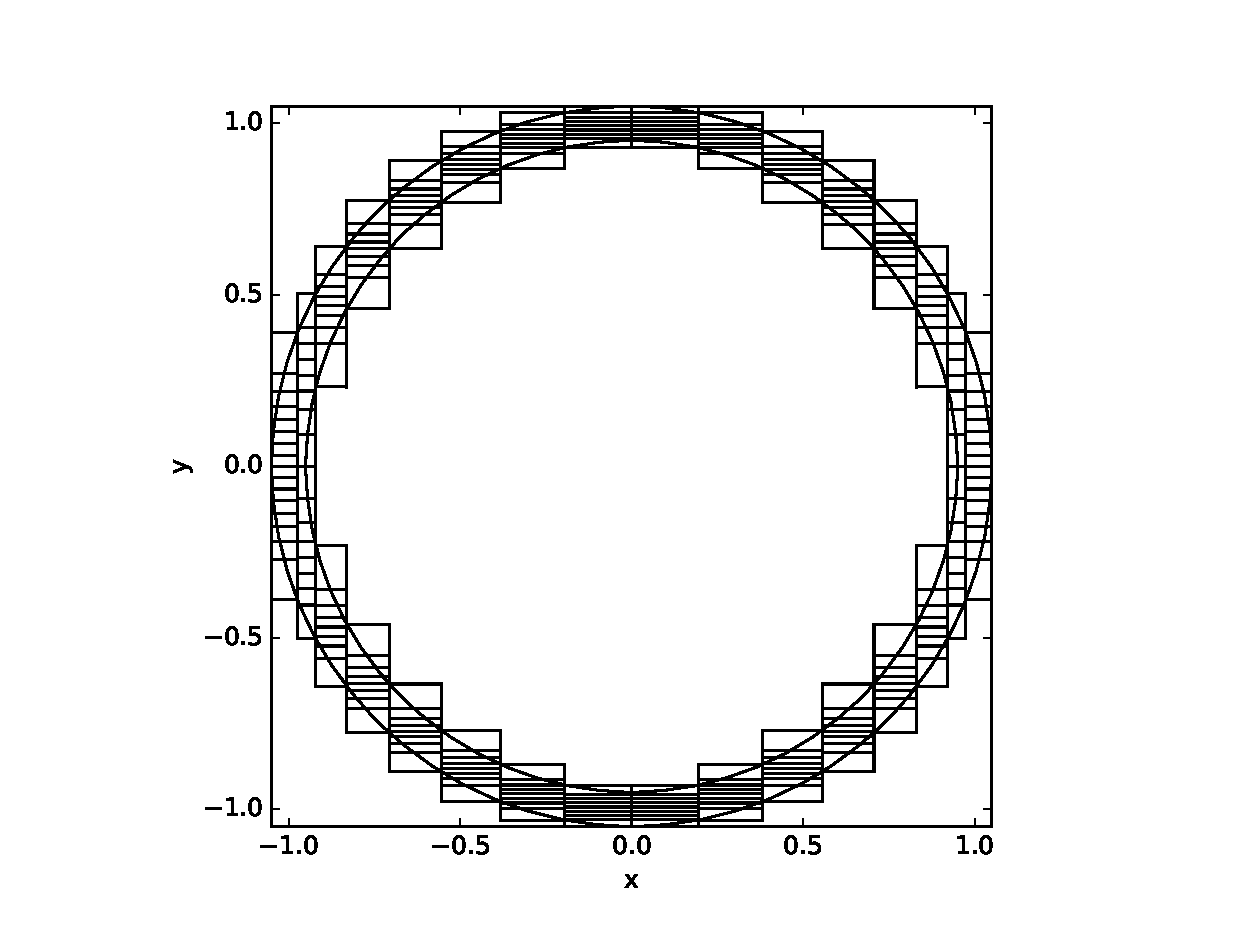
\includegraphics[width=8cm,clip]{./fig/domain_cart.eps}
  \caption{Schematic figure of domain decompostion by the multisection
    method in x-y coordinate. Domains are divided by 16x8.}
  \label{fig:domain_cart}
\end{figure}

\begin{figure}
  \centering
    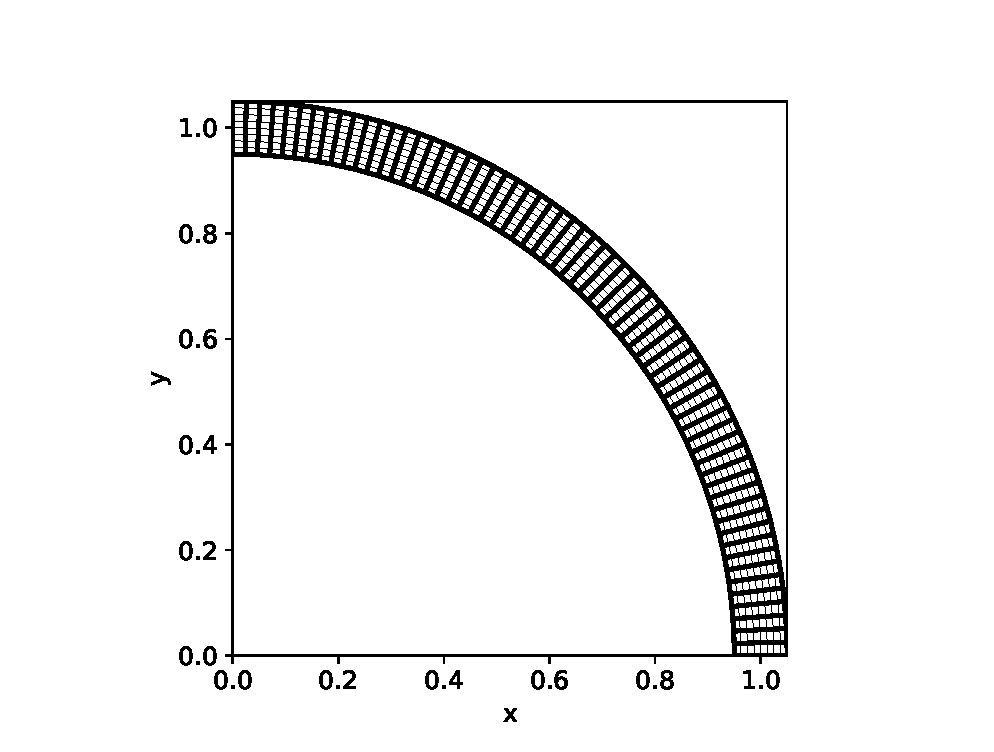
\includegraphics[width=8cm,clip]{./fig/domain_cyl.eps}
  \caption{Schematic figure of domain decompostion by the multisection
    method in cylindrical coordinate. Domains are divided by 4x32.}
  \label{fig:domain_cyl}
\end{figure}

In original implementation, a logical structure of the tree cells and
computational domains are calculated on a Cartesian
coordinate. However, the Cartesian coordinate is not suitable for the
global planetary ring simulations. We can see this reason from
Figure~\ref{fig:domain_cart} which gives an example of domain
decomposition by 16 $\times$ 8 on the Cartesian coordinate for a
quadrant of a ring with the radius of 1.0 and the width of 0.1.

Domains have various shape and some of them have high aspect ratio.
The domains at $x \sim 0$ are elongated along the x direction. On the
other hand, the domains at $x \sim 1$ are elongated along the y
direction. However, the domain shapes at $x \sim 0$ and $x \sim 1$ are
not 90-degree rotation symmetric because of the nature of the
multisection method.

The wide variation of the domain shapes means that tree structure and
the length of the interaction list are the largely different for
different processes. Thus it is difficult to achieve a good load
balance. In addition, the high aspect ratio of the domain increases
the communication costs, because the costs is roughly proportional to
the area of the surface of the domain.

In the point of view of the load balance and communication cost, the
ideal case is that the shapes of all domains are the same
squares. Unfortunately, as long as we use the Cartesian coordinate,
the ideal decomposition is difficult because of the curvature of the
ring.

To approach the ideal domain decomposition, we introduce a cylindrical
coordinate ($r$, $\phi$, $z$). We replace $x$ and $y$ with $\phi$ and
$r$. In this coordinate, a distance between two separate points $ds$
is defined by
\begin{equation}
  \label{eq:metric}
  ds^2 = dx^2 + dy^2 + dz^2 \sim d\phi ^2 + dr^2 + dz^2.
\end{equation}

Figure~\ref{fig:domain_cyl} is the same as
figure~\ref{fig:domain_cart}, but decomposed by 4 $\times$ 32 by using
the cylindrical coordinate. Each domains have almost the same square
shapes. It means the good load balance and the decreasing
communication costs compared to those on the Cartesian coordinate.

We also introduce this coordinate to the tree structure: We use the
cylindrical coordinate for constructing the tree, LET and the
interaction lists. On the other hand, for the calculation of the
multiple moment of the tree cell and the interaction calculation, we
use the position defined by the Cartesian coordinate.

For large $\phi$, the approximation of equation~\ref{eq:metric} is
broken and the distance is overestimated. For example, at $\phi=\pi$,
the approximation distance is overestimated by 57 \%. This
approximation means that the accuracy of the force evaluated by
multipole approximation from distant particles is somewhat
worse. However, since the ring system is roughly one-dimensional
structure, the contributions from distant tree cell decreases as
$\phi^{-1}$. Thus our approximation dose not cause serious problem.

\subsection{Exchange Particles}
\label{subsec:exptcl}

Before the construction of the local tree, particles should migrate so
that they belong to appropriate domains. In a reference frame, the
particle move a large distance for multiple timesteps. It means most
particles should go to other domains. It could increase the
communication cost. However, in a rotating frame with the typical
angular speed of the ring, most particles do not seem to move a large
distance. Thus, before the exchange particle, we counter-rotate
particles by the same angle as the typical rotation angle of the ring.

If the particles exactely move on Kepler orbit around the planet, the
number of particles to be sent from each domain is estimated by a
following equation.

\begin{eqnarray}
  n_{send} &=& n\int_{r_0}^{r_1} {\rm min}(|\Delta v_k(r) \Delta t|, l) dr, \\
  v_k(r) &=& \sqrt{\frac{Gm}{r}}, \\
  \Delta v_k(r) &=& v_k(r) - v_k(a),
\end{eqnarray}
where $n$ is the surface number density $r_0$ and $r_1$ are the radii
of the inner and outer edge of the domain, $l$ is the length of the
domain in the $\phi$ direction, $\Delta t$ is the time interval
between the exchange particles procedures, $m$ is the mass of the
planet and $a$ is the typical ring radius. In this paper, we set $a$
to be the distance between the planet and the middle of the ring
width.

If $|\Delta v_k(r) \Delta t| > l$, all particles at $r$ should go to
other domains. In other words, we should chose $\Delta t \lesssim
\frac{2al}{|r-a| V_k(a)}$. If we think the shape of the domain is
square, we can also write the above condition as $\Delta t \lesssim
\frac{2a}{|r-a| V_k(a)}\sqrt{\frac{2\pi w}{n_p}}$, where $w$ is the
width of the ring and $n_p$ is the number of processors.

\subsection{Exchange Local Essential Tree}
\label{subsec:exlet}

\begin{figure}
  \centering 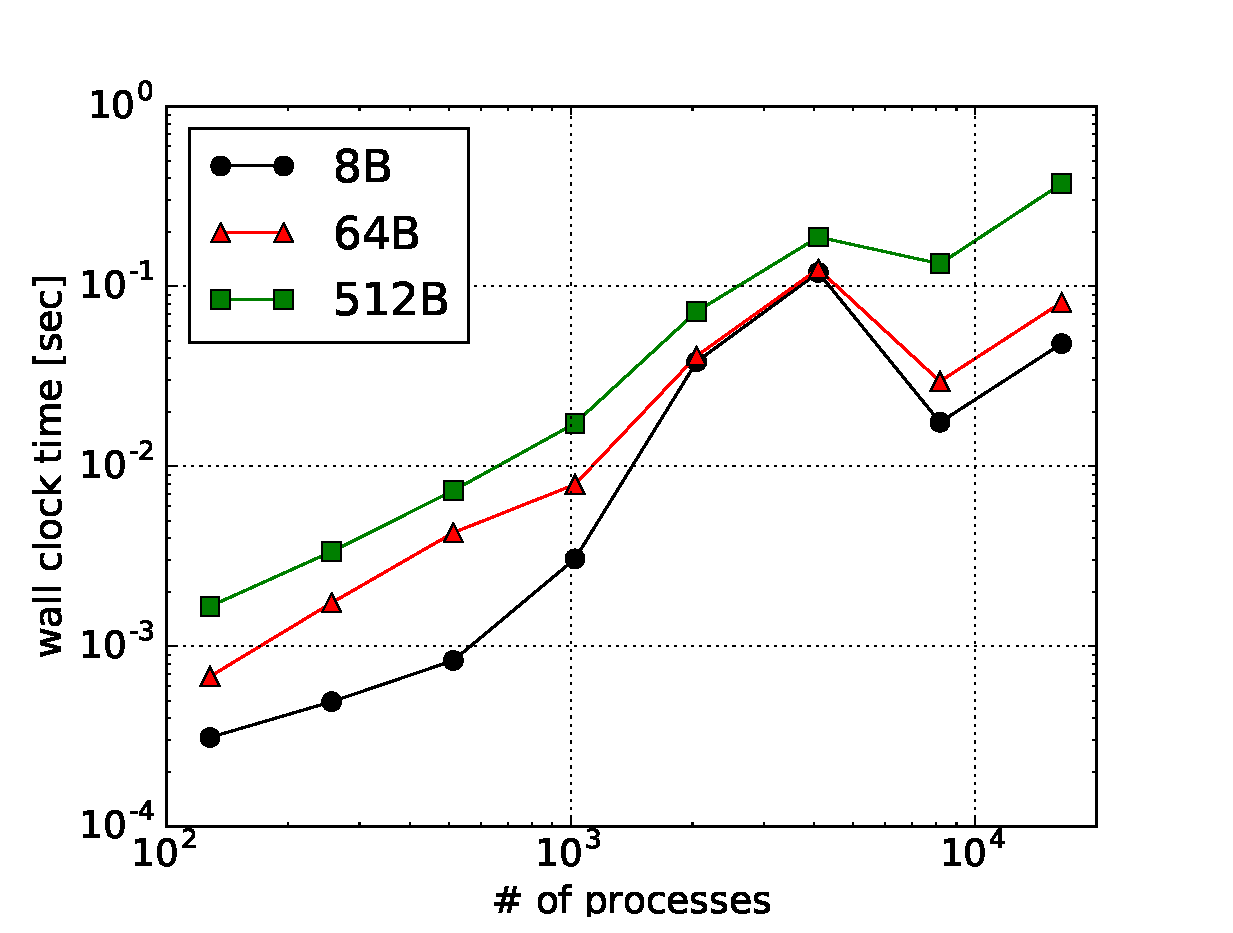
\includegraphics[width=8cm,clip]{./fig/comm_np-wtime.eps}
  \caption{Wall clock time for {\tt MPI\_Alltoall} against the number of processors.}
  \label{fig:comm_np-wtime}
\end{figure}

\begin{figure}
  \centering
  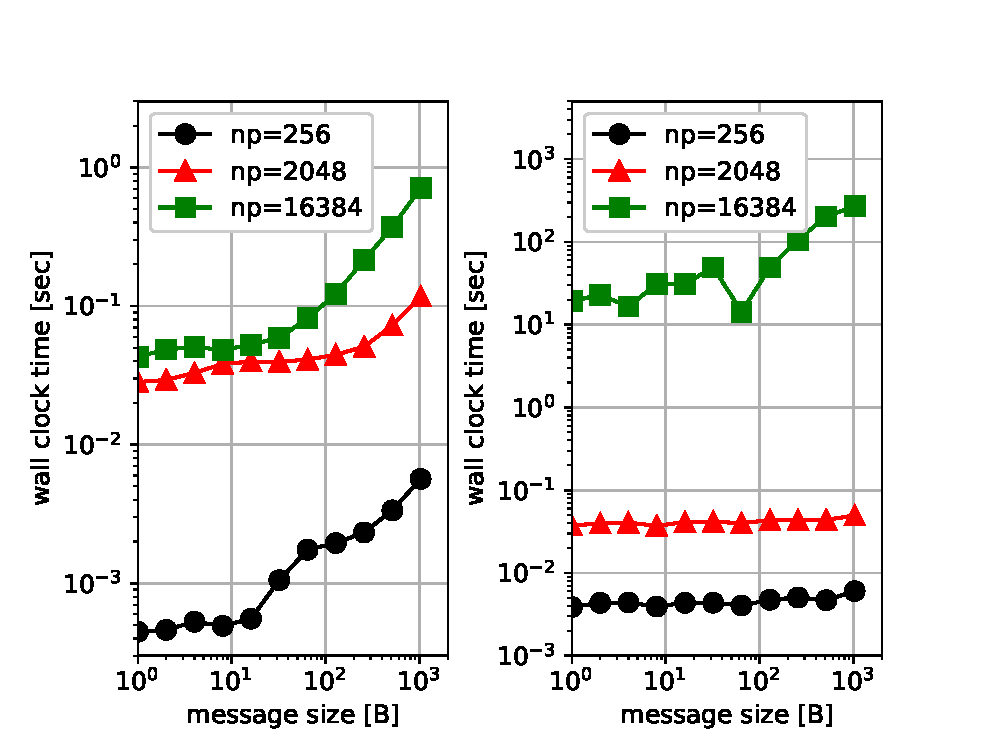
\includegraphics[width=8cm,clip]{./fig/comm_msize-wtime.eps}
  \caption{Wall clock time for {\tt MPI\_Alltoall} against the size of the message sent per process.}
  \label{fig:comm_msize-wtime}
\end{figure}

In the original implementation of the exchange LET, each domain
measure the distances from all other domains and exchange LETs among
all processes. This communication is realized by {\tt
  MPI\_Alltoall(v)}.

%On many systems, {\tt MPI\_Alltoall(v)} is suboptimal and we should
%avoid do use this.

Figures~\ref{fig:comm_msize-wtime} and \ref{fig:comm_msize-wtime} show
the wall clock time of {\tt MPI\_Alltoall} against the number of
processes and the size of the sent message per process,
respectively. The wall clock time is super linear against the number
of processors. We can also see that the wall clock time is constant up
to rather large message size ($\sim$ 100 Byte). It means we have to
avoid {\tt MPI\_Alltoall} communication among all processors.

To avoid all-to-all communication among all processes, we introduce a
kind of the tree structure to the domain structure. In principle, if
we have the tree of domains, the all-to-all communication among all
processes is not needed because each process dose not need the
multipole moments from distant domains individually, but only needs
locally combined multipole moment from distant domains.

For simplicity, in our method, we consider the original domain
structure by the multisection methods as the tree structure with the
depth of two. In other words, the root cell of the domain tree has
$n_x$ sub-cells (hereafter, call it ``super domain'') and each
sub-cell (``super domain'') has $n_y$ sub-sub-cells (we do not divide
domains in the $z$ direction because the thickness of the ring is very
thin). Here $n_x$ and $n_y$ are the number of processes in the $x$ and
$y$ directions, respectively.

The steps of the exchange LET with the super domain method is as
follows.

\begin{enumerate}

\item Process with the r-index of zero (hereafter, call it super
  process) gather LETs of the top tree cells in the r-direction.

\item Super process combines the multipole moment from received LETs.

\item Super process gathers the combined multipole moments from other super
  domains by using {\tt MPI\_Allgather}.

\item Super process broadcasts the combined multipole moments in r-direction.

\item Process measures the distances between own super domain and
  other super domains.

  %\begin{enumerate}
  \begin{description}
    
  \item{(a1)} If the distance is far enough, do nothing because this process
    already received LET from the target super domain at step 3.
  
  \item{(b1)} Otherwise, each process make LETs for the target super domain
    and send the LETs to the process with the same $r$-index in the
    target super domain by {\tt MPI\_Isend/recv}.

  \item{(b2)} Each process broadcast the received LETs in the $r$
    direction.

  \end{description}
    
  %\end{enumerate}
  
\end{enumerate}

If we use this methods, we can completely remove {\tt
  MPI\_Alltoall(v)}.



\subsection{Load Balance of Force Kernel on Manycore Processor}
\label{subsec:force}

The interactions are calculated on 64 CPEs in parallel. In our
implementation, different CPEs read different interaction lists and
calculate their interactions. Thus we can avoid reduction of the
forces between CPEs.

To achieve a good load balance, the length of the interaction list on
CPEs should be the same. However, it is difficult to obtain the
optimal solution in a reasonable time. Instead of this, we obtain an
approximated solution by the greedy algorithm. Our implementation is
as follows.

\begin{enumerate}
  
\item Sort the interaction lists by its length.

\item Assign the first 64 lists on 64 CPEs, one-by-one.

\item Assign the next interaction list on the CPE with the shortest
  total interaction list.

\item Repeat step 3 until all lists are assigned on CPEs.

\end{enumerate}
  
Note, at step 3, to find the CPEs with the shortest interaction list,
we use binary tree algorithm.

The solution obtained by this method dose not guarantee the optimal
one. However, unless the distribution of the interaction lists length
is very peculiar (e.g. except for one interaction list, all
interaction list length is one), the approximated solution is very
close to the optimal one.

\section{Performance Results}
\label{sec:result}

In this section, we describe the initial ring model and the measured
performance. 

\subsection{Initial Condition}

As an initial model, we make a ring with the radius of 1.0, the width
of 0.01 and the optical depth $\tau$ of 1.0. All particles are
identical and their radii are the same as the Roche radius. We put
particles on three layers. We put 3/$N$ particles on a regular grid on
each layer. The grids are shifted by half grid size grid to the grids
of neighbor layers. The all particles are on Kepler orbit.

\subsection{Interaction Model}

In our simulations, since $\tau$ is unity, the particles collide with
each other frequently. Since the radius of the particle is the Roche
radius, when the particles collide, the particles rather rebound than
gravitational accreation. To handle this nature of collision, we
regard a particle as a soft sphere. In this model, we consider not
only the gravitational force, but also both a spring and a dashpot
forces. Equation \ref{eq:interaction} gives the definition of the
particle-particle interaction.

\begin{eqnarray}
  \bm F_{ij} = \left \{
  \begin{array}{ll}
     G \frac{m_i m_j}{r_{ij}^3} \bm r_{ij} & \left(r_{ij} > r_{\rm coll} \right) \\
     \left[  G \frac{m_i m_j} {r_{\rm coll}^3} + \frac{m_j}{m_i + m_j} \left( \kappa \frac{ r_{ij} - r_{\rm coll}}{r_{ij}} + \eta \frac{\bm r_{ij} \cdot \bm v_{ij}}{r_{ij}^2} \right) \right] \bm r_{ij} & \left( r_{ij} \le r_{\rm coll} \right)
  \end{array}
  \right.
  \label{eq:interaction} 
\end{eqnarray}

with $\bm r_{ij} = \bm r_j - \bm r_i$, $\bm v_{ij} = \bm v_j - \bm
v_i$, $r_{ij} = \| \bm r_{ij} \|$. Here, ${\mathbf F_{ij}}$ is the
acceleration particle $i$ due to particle $j$, ${\mathbf r_{ij}}$ and
${\mathbf v_{ij}}$ are the relative position and velocity vectors, $G$
is the gravitational constant (taken to be unity in this paper), $m_i$
is the mass of particle $i$, $r_{coll}$ is the distance at which two
particles collide, and $\eta$ and $\kappa$ are parameters which
determine the coefficient of restitution. We chose these parameters so
that the coefficient of restitution in radial direction is 0.5.

Particle-particle interaction consists of 9 multiplications, 8
additions, and one square root and one division
operations. Instruction set of Sunway 26010 processor does not include
fast approximation for neither square root or reciprocal square
root. So we implemented fast initial guess and high-order convergence
iteration in software. The number of operations in this part is 7
multiplications, 5 additions and two integer operations. Therefore,
for particle-cell interactions the number of floating-point operations
is 31, and for particle-particle interactions, which include the
repulsive force during physical collisions, is 47. The total number of
floating-point operations is obtained by counting the number of
interactions calculated and multiply them with these number of
floating-point operations per interaction. We ignore all operations
other than the interaction calculation, since as far as the number of
floating-point operations is concerned, that for interaction
calculation is more than 99\% of total operation count.

\subsection{Numerical Method}

We use the Barnes-Hut tree method using modified FDPS including the
algorithms described above. The opening criterion of the tree $\theta$
is 0.5. The integration method is leap frog with the shared timestep
of $1/128$. We use the same interaction list for 64 steps.

In the ring simulation the global structure is not drastically changed
for rotation period. Thus the domain decomposition is done once at the
beginning and we do not include the time for the domain decomposition.


\subsection{Performance}

To measure the performance, we measure the time for 64 timesteps,
including the time for diagnostics. The execution time is measured by
the MPI wallclock timer, and operation count is from the counted
number of interactions calculated.

For the weak-scaling measurement, we have performed runs with 1M
particles per MPI process and for the strong-scaling measurement, the
total number of particles is 2G.

\begin{figure}
  \centering
    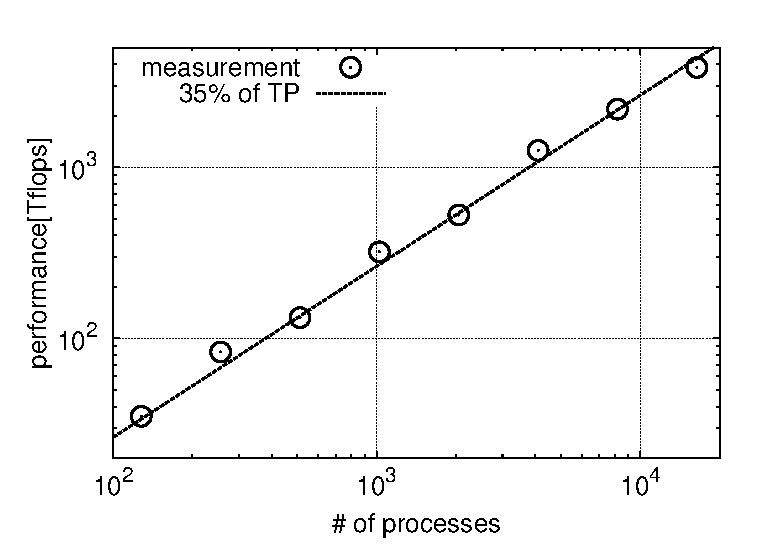
\includegraphics[width=8cm,clip]{./fig/weak_speed.eps}
  \caption{Performance in tera flops for weak-scaling test. The number
    of particles per process is 1M. Solid line indicates 35 \% of the
    theoretical peak performance of TaihuLight. Open circles indicate
    measured performance.}
  \label{fig:weakpf}
\end{figure}

\begin{figure}
  \begin{center}
    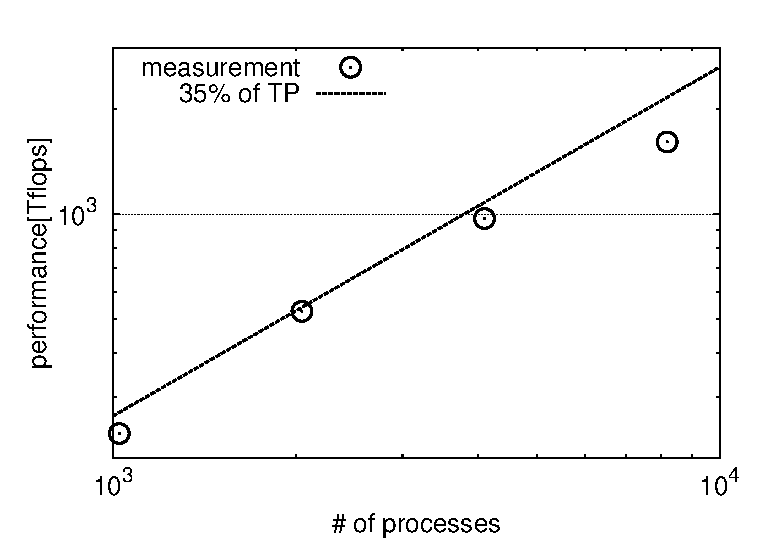
\includegraphics[width=8cm,clip]{./fig/strong_speed.eps}
  \end{center}
  \caption{Performance in tera flops for stron-scaling test. The
    number of particles per process is 2048M. Solid line indicates 35
    \% of the theoretical peak performance of TaihuLight. Open circles
    indicate measured performance.}
  \label{fig:strongpf}
\end{figure}

\begin{figure}
  \begin{center}
    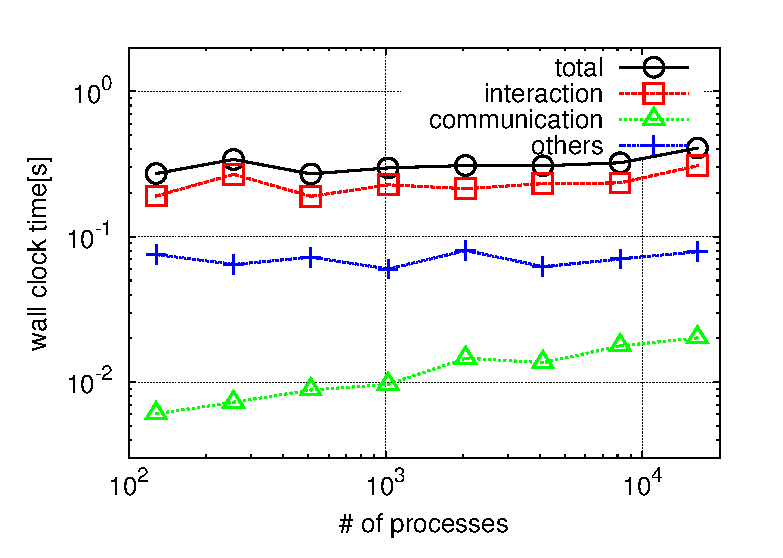
\includegraphics[width=8cm,clip]{./fig/weak.eps}
  \end{center}
  \caption{Time per timestep for weak-scaling test. The number of
    particles per process is 1M.}
  \label{fig:weak}
\end{figure}

\begin{figure}
  \begin{center}
    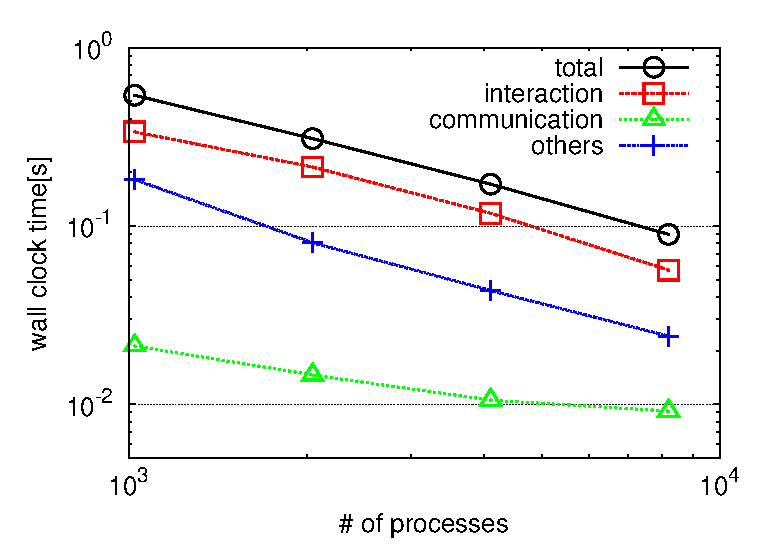
\includegraphics[width=8cm,clip]{./fig/strong.eps}
  \end{center}
  \caption{Time per timestep for strong-scaling test. The total number of
    particles is 2048M.}
  \label{fig:strong}
\end{figure}

Figures \ref{fig:weakpf} and \ref{fig:strongpf} show the speed in tera
flops, for both the strong and weak scaling measurements. We can see
that the weak scaling performance is quite good. The performance of
run for 8G particles on 8192 nodes is 2.18 PFlops, or 35\% of the
theoretical peak performance of the Sunway TaihuLight system. Since
our main scientific target is runs with very large number of particles
which has been impossible, weak-scaling performance is our main
interest.

Figures \ref{fig:weak} and \ref{fig:strong} show the time per one
timestep, for both the strong and weak scaling measurements. The most
intensive part is the interaction calculation. From Figures
\ref{fig:weakpf}, the time for communication increase slower than
linear increase. It means we can remove the bottleneck from {\tt
  MPI\_Alltoall(v)}.

Table~\ref{tab:break_down} shows the breakdown in the case of
weak-scaling test on 8192 nodes. The second and the third column show
the time of the first step and the averaged time over 64 steps for
each operation. The forth column shows the values in the second column
divided by those in the third column. Roughly speaking, these values
indicate the speedup factor when we use the persistent list method.

We find that if we use the persistent list method, the total time
becomes 5.3 times faster.

The ``Local Tree update'' and the ``Global Tree update'' is the time
for updating the physical quantities of the tree cell of the local
tree and the global tree, respectively. These times become slightly
faster. This is because these time include not only the time for
calculating multipole moment of the tree cell, but also the time for
updating tree cell boundaries. However, the tree cell boundaries is
used only for the tree traverse. Thus, we skip updating boundaries at
all steps other than the first step.

Others mainly include the data copies. The number of data copies also
reduce if we use the persistent list method.


\begin{table}
  \caption{Break down}
  \label{tab:break_down}
  \begin{tabular}{lccc}
    \toprule
    Operation & first step & 64 averaged & speedup\\
    \midrule
    exchange Particles            & 0.308   & 0.00481  & 64.0 \\
    Local Tree construction       & 0.0568  & 0.000888 & 64.0 \\
    Local Tree update             & 0.0195  & 0.0130   & 1.5 \\
    LET construction              & 0.00416 &  $6.50 \times 10^{-5}$  & 64.0 \\
    LET communication             & 0.0238  & 0.0128   & 1.86 \\
    Global Tree construction      & 0.178   & 0.0141   & 12.6 \\
    Global Tree update                 & 0.0273  & 0.0165   & 1.65 \\
    Interaction List construction & 0.657   & 0.0103   & 64.0 \\
    Interaction calculation       & 0.285   & 0.235    & 1.21 \\
    Others                        & 0.150   & 0.0156   & 9.62 \\
    \midrule
    Total                         & 1.71   & 0.323     & 5.29 \\
  \bottomrule
  \end{tabular}
\end{table}

\section{Summary and Discussion}

\subsection{Real Size Ring Simulation}

As we see in section 1, to investigate the ring structure, we need
$10^{16}-10^{19}$ particle steps. With our code, We can integrate
about $3.2 \times 10^6$ particles per second per process. In other
words we need $8.7 \times 10^5 - 8.7 \times 10^8$ process hours. If we
can use nearly full node of Sunway TaihuLight or other super computers
with similar peak performance, the simulations would be finished
within the reasonable time. In near future, we will perform these
simulations.

\subsection{Extension of Proposed Algorithms}

The persistent list methos is based on the nature of the ring system
which is the velocity dispersion of the system is very low so that the
particle relative positions keep almost the same for multiple
timesteps. Thus we can use this methods applied SPH, MD or DEM
simulations.

This method is also useful $N$-body+SPH simulation such as galaxy
formation simulations. This is because the timestep of the simulation
is determined by SPH particles not by $N$-body particles with high
velocity dispersion.

The super domain method (or introducing tree structure to the domain
structure) would become necessary methods in the future. This is
because optimization of all-to-all communication is difficult and the
communication time linearly increases as the number of processes, at
least. It means, if the number of processes is comparable with the
number of particles per process, the communication time could become
dominant part in the total execution time.

In this paper, we use only level-two tree structure. This methods is
good enough for our aim. However, if we use more processes we might
need to introduce more general tree structure to the domain
decomposition. We will study it in near future.

\subsection{Summary}

In this paper, we described the algorithms and performance of a highly
efficient simulation code for self-gravitating planetary rings on the
Sunway TaihuLight system. We mainly develop five new algorithms: 1)
Persistently use the same interaction list for multiple timesteps. 2)
Use the cylindrical coordinate for constructing the domain and the
tree logical structure. 3) Counter rotate particles for decreasing
communication costs for exchange particles. 4) Introduce the super
domain to remove all-to-all communication for exchange LET. 5) Load
balance for the interaction calculation by the greedy algorithm. We
implement these algorithms to FDPS and we achieve 2.18 PFlops, or 35
\% of the theoretical peak on 8192 processes. It means we are ready to
perform real size ring simulation. In near future, we will try to
perform these simulations to investigate the formation of the
planetary ring.

\appendix

\section{Force Kernel Tuning on SW21060}

Since the force kernel is the most intensive part in $N$-body
simulation, we need fast force kernel. Different CPEs calculate
different i-particle groups. At first, each CPE stores 256 i-particles
and 4 j-particles to its local memory. Then CPE calculate forces on
256 i-particles from 4 j-particles. To hidden the latency of reading
j-particles, during force calculation, next 4 j-particles are stored
with DMA.

For tuning on the force kernel itself, we develop it in assembly
language because the optimization by the compiler is limited. In
addition, instruction set of Sunway 26010 processor does not include
fast approximation for neither square root or reciprocal square
root. So we implemented fast initial guess and high-order convergence
iteration in software.

\section{Sort on SW21060}

The sorting in the particles frequently used in our code. For example
for the tree construction, we sort the particles by their Morton key.
In original implementation of FDPS, we used the radix sort for the
Morton key sort. The radix sort is easily parallelized and is known
one of the fastest sort on GPUs.

The bottleneck of the radix sort is the bandwidth of the main memory.
The bandwidth of SW21060 processor is about ten times slower than that
of the current GPU, such as GTX1080. Thus the radix sort is not
optimal choice on SW21060.

Instead of radix sort, we used so-called sample-sort method. The steps
of sample sort s as follows.

\begin{enumerate}
  
\item Sample elements randomly and store them to the local memory.

\item Sort the samples by quick sort on single core.

\item Find the partition to split the sample into 64 segments
  equivalently and assign 64 segments to 64 CPEs one-by-one.

\item Store elements from original array to appropriate local memory.

\item Sort the elements by quick sort on each CPEs.
  
\end{enumerate}

In this method, once we store elements to the local memory, CPEs do
not need to access to the main memory, until the sort is done. Thus
the main memory bandwidth is not serious issue.

%\begin{thebibliography}{1}

%\bibitem[Ballouz et al.(2017)]{Ballouzetal2017} Ballouz, R.-L., Richardson, D.~C., \& Morishima, R.\ 2017, \aj, 153, 146  
  
%\bibitem[Barnes \& Hut(1986)]{BarnesHut1986} Barnes, J., \& Hut, P.\ 1986, \nat, 324, 446
  
%\bibitem[Barnes(1990)]{Barnes1990} Barnes, J.~E.\ 1990, Journal of Computational Physics, 87, 161

%\bibitem[B{\'e}dorf et al.(2012)]{Bedorfetal2012} B{\'e}dorf, J., Gaburov, E., \& Portegies Zwart, S.\ 2012, Journal of Computational Physics, 231, 2825

%\bibitem[B{\'e}dorf et al.(2014)]{Bedorfetal2014} B{\'e}dorf, J., Gaburov, E., Fujii, M.~S., et al.\ 2014, Proceedings of the International Conference for High Performance Computing, Networking, Storage and Analysis, p.~54-65, 54
  
%\bibitem[Hamadaetal(2009)]{Hamadaetal2009} Hamada, T., Narumi, T., Yokota, R., Yasuoka, K., Nitadori, K., \& Taiji, M.\ 2009, Proceedings of the Conference on High Performance
%  Computing Networking, Storage and Analysis, 62, 12
  
%\bibitem[Iwasawa et al.(2016)]{Iwasawaetal2016} Iwasawa, M., Tanikawa, A.,
%  Hosono, N., et al.\ 2016, \pasj, 68, 54

%\bibitem[Ishiyama(2014)]{Ishiyama2014} Ishiyama, T.\ 2014, \apj, 788, 27
  
%\bibitem[Makino(1991)]{Makino1991c} Makino, J.\ 1991, \pasj, 43, 621

%\bibitem[Michikoshi \& Kokubo(2017)]{MichikoshiKokubo2017} Michikoshi, S., \& Kokubo, E.\ 2017, \apjl, 837, L13

%\bibitem[Rein \& Latter(2013)]{ReinLatter2013} Rein, H., \& Latter, H.~N.\ 2013, \mnras, 431, 145

%\bibitem[Rein \& Liu(2012)]{ReinLiu2012}, H. {Rein} \& S.-F. {Liu}, 2012, \aap, 537, 128

%\bibitem[Stadel(2001)]{Stadel2001} Stadel, J.~G.\ 2001, Ph.D.~Thesis, 3657
  
%\bibitem[Wisdom \& Tremaine(1988)]{WisdomTremaine1988} Wisdom, J., \& Tremaine, S.\ 1988, \aj, 95, 925
  
%\bibitem[Zebker et al.(1985)]{ZEBKER1985531} Zebker, H.~A., Marouf, E.~A., \& Tyler, G.~L.\ 1985, \icarus, 64, 531

%\bibitem{2012AJ....143...72M} Mamajek, E.~E., Quillen, A.~C., Pecaut,
%  M.~J. et al.: Planetary Construction Zones in Occultation: Discovery
%  of an Extrasolar Ring System Transiting a Young Sun-like Star and
%  Future Prospects for Detecting Eclipses by Circumsecondary and
%  Circumplanetary Disks.  \aj, 143, 72, (2012)

%\bibitem{2014MNRAS.441.2845V} van Werkhoven, T.~I.~M., Kenworthy,
%  M.~A., \& Mamajek, E.~E.: Analysis of 1SWASP J140747.93-394542.6
%  eclipse fine-structure: hints of exomoons. \mnras, 441, 2845, (2014)

%\bibitem{2015MNRAS.446..411K} Kenworthy, M.~A., Lacour, S., Kraus, A.,
%  et a.: Mass and period limits on the ringed companion transiting the
%  young star J1407. \mnras, 446, 411, (2015)

%\bibitem[Kenworthy \& Mamajek(2015)]{2015ApJ...800..126K} Kenworthy,
%  M.~A., \& Mamajek, E.~E.\ 2015, \apj, 800, 126
  
%\end{thebibliography}

\bibliographystyle{plain}
\bibliography{reference}

\end{document}
